\documentclass[svgnames,11pt]{beamer}
\input{/home/tof/Documents/Cozy/latex-include/preambule_commun.tex}
\input{/home/tof/Documents/Cozy/latex-include/preambule_beamer.tex}
%\usepackage{pgfpages} \setbeameroption{show notes on second screen=left}
\author[]{Christophe Viroulaud}
\title{TP qualité du vin\\Algorithme kNN}
\date{\framebox{\textbf{Algo 07}}}
%\logo{}
\institute{Première - NSI}

\begin{document}
\begin{frame}
\titlepage
\end{frame}
\begin{frame}
    \frametitle{}

    
    \begin{center}
    \centering
    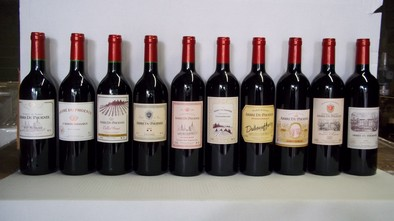
\includegraphics[width=8cm]{ressources/vins.jpg}
    \captionof{figure}{\centering Les propriétés chimiques d'un vin influencent grandement sur sa qualité.}
    \end{center}

\end{frame}
\begin{frame}
    \frametitle{}

\begin{center}
\centering
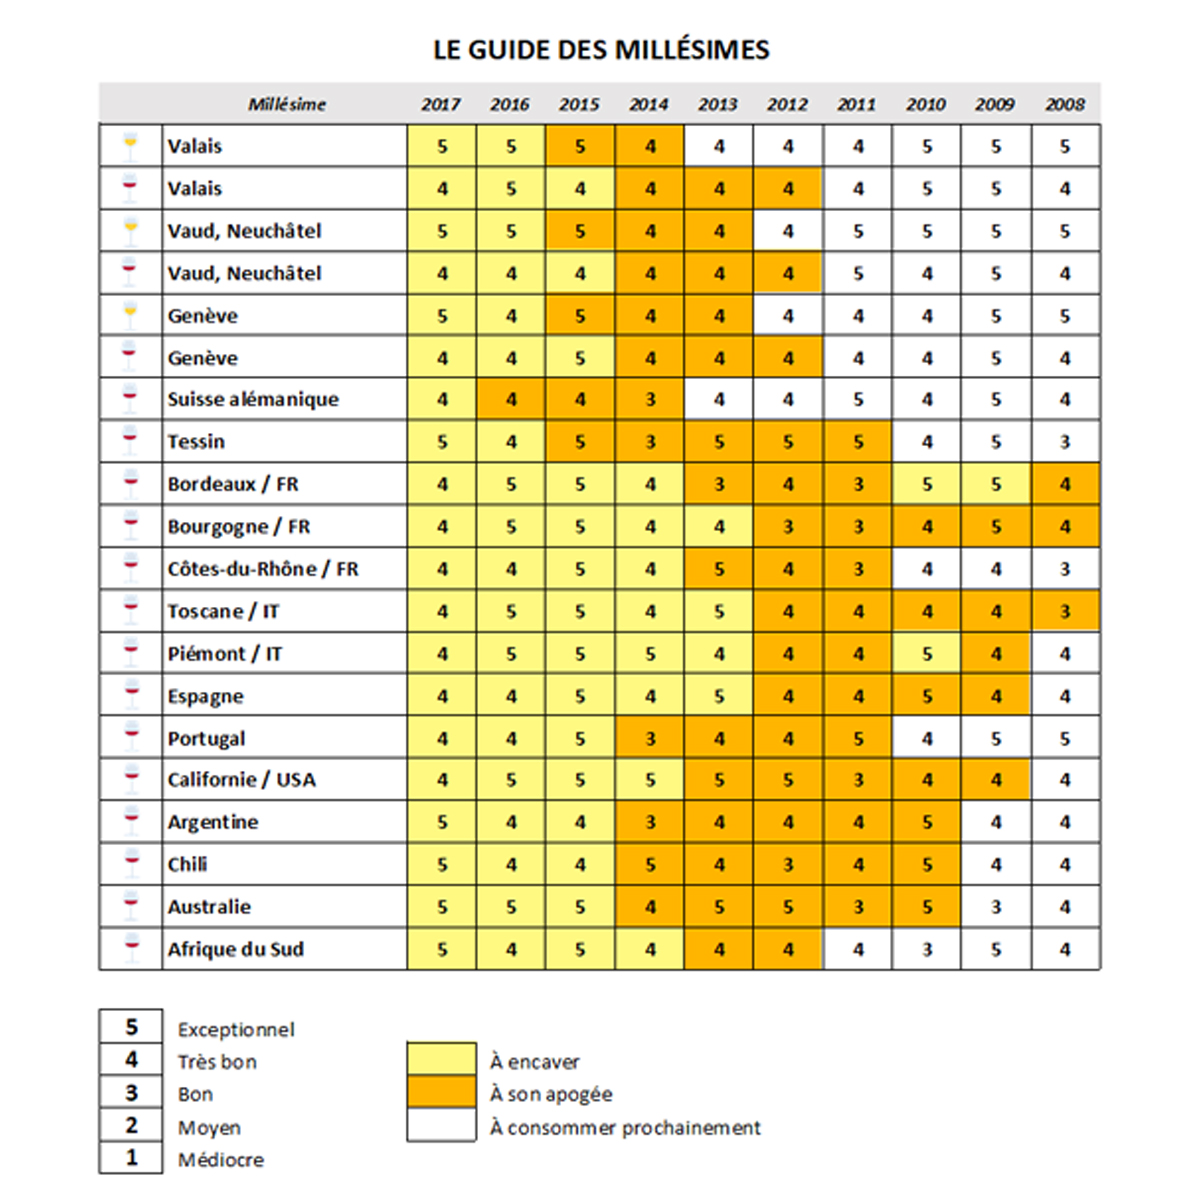
\includegraphics[width=8cm]{ressources/classement.jpg}
\captionof{figure}{\centering Les œnologues établissent des classements des vins.}
\label{IMG}
\end{center}
    

\end{frame}
\begin{frame}
    \frametitle{}

    \begin{framed}
        \centering Établir un algorithme de classement des vins en fonction de leur propriétés chimiques.
    \end{framed}

\end{frame}
\section{Études des données}
\begin{frame}
    \frametitle{Études des données}

    On dispose d'un jeu de données sur plusieurs propriétés de différents vins:
    \begin{itemize}
        \item fixed acidity
        \item volatile acidity 
        \item citric acid
        \item residual sugar
        \item chlorides
        \item free sulfur dioxide
        \item total sulfur dioxide
        \item density
        \item pH
        \item sulphates
        \item alcohol
    \end{itemize}

\end{frame}
\begin{frame}
    \frametitle{}

    \begin{aretenir}[Observation]
        De plus chaque vin a obtenu une note (\textbf{\texttt{quality}}) entre 1 et 8. Les données sont donc \textbf{étiquetées}.
    \end{aretenir}
\begin{activite}
\begin{enumerate}
    \item Télécharger et extraire l'annexe \textbf{\texttt{winequality-red.zip}} sur le site \url{https://cviroulaud.github.io}
    \item Ouvrir le fichier \textbf{\texttt{winequality-red.csv}} avec un tableur pour observer les données.
\end{enumerate}
\end{activite}
\end{frame}
\begin{frame}
    \frametitle{}

    \begin{aretenir}[Observation]
        Lors de l'étude des iris, 2 caractéristiques seulement (longueur et largeur des pétales) étaient observées. Il était donc possible de les représenter graphiquement.\\
        Les vins possèdent 11 propriétés différentes; une représentation graphique est donc impossible.
    \end{aretenir}

\end{frame}
\section{Algorithme kNN}
\subsection{Principe}
\begin{frame}[fragile]
    \frametitle{Algorithme kNN - Principe}

    On dispose des propriétés d'un vin:
\begin{center}
\begin{lstlisting}[language=Python , basicstyle=\ttfamily\small, xleftmargin=0.2em, xrightmargin=0em]
vin_inconnu = {'fixed acidity': 6.9, 'volatile acidity': 0.5, 'citric acid': 0.19, 'residual sugar': 3.9, 'chlorides': 0.16, 'free sulfur dioxide': 31.0, 'total sulfur dioxide': 50.0, 'density': 0.994, 'pH': 3.01, 'sulphates': 0.61, 'alcohol': 9.3}
\end{lstlisting}
\end{center}
Et on cherche à déterminer une note (\textbf{\texttt{quality}}) en établissant un modèle dans le jeu de données fourni.
\end{frame}
\begin{frame}
    \frametitle{}

L'algorithme est similaire à celui utilisé pour les iris:
\begin{itemize}
    \item Charger les données dans le programme.
    \item Choisir k.
    \item Stocker les propriétés du vin inconnu.
    \item Calculer la distance euclidienne entre le vin inconnu et tous les autres vins.
    \item Trier les vins selon leurs notes.
    \item Sélectionner les \emph{k} plus proches vin (en distance) du vin inconnu.
    \item Affecter la note majoritaire des \emph{k} plus proches vins (en distance) au vin inconnu.
\end{itemize}

\end{frame}
\subsection{Importation des données}
\begin{frame}
    \frametitle{Importation des données}
\begin{activite}
\begin{enumerate}
    \item Créer le fichier \textbf{\texttt{qualitevin.py}} dans le même dossier que le fichier \textbf{\texttt{csv}}.
    \item Importer les données des vins dans le programme.
    \item Créer un tableau \textbf{\texttt{vins}} de dictionnaires. Chaque dictionnaire représentera un vin du fichier \textbf{\texttt{csv}}. Toutes les propriétés seront converties en nombre flottant sauf \textbf{\texttt{quality}} qui sera converti en entier.
\end{enumerate}
\end{activite}
    

\end{frame}
\begin{frame}
    \frametitle{Avant de regarder la correction}
\begin{center}
    \centering
    \includegraphics[width=3cm]{/home/tof/Documents/Cozy/latex-include/stop.png}
    \end{center}
{\Large
    \begin{itemize}
        \item Prendre le temps de réfléchir,
        \item Analyser les messages d'erreur,
        \item Demander au professeur.
    \end{itemize}
}
\end{frame}
\begin{frame}[fragile]
    \frametitle{Correction}

\begin{center}
\begin{lstlisting}[language=Python , basicstyle=\ttfamily\small, xleftmargin=0.2em, xrightmargin=0em]
fichier = open(f, encoding="utf8")
data = csv.DictReader(fichier)

vins = []
for v in data:
    vin = {}
    for attribut, valeur in v.items():
        # qualité est le seul entier
        if attribut == "quality":
            vin[attribut] = int(valeur)
        else:
            vin[attribut] = float(valeur)
    vins.append(vin)

fichier.close()
\end{lstlisting}
\end{center}

\end{frame}
\subsection{Distance}
\begin{frame}
    \frametitle{Distance}

Même si les données ne sont pas représentables graphiquement, il est possible de calculer la distance euclidienne entre deux vins:
$$distance =$$
$$(fixed acidity_{connu}-fixed acidity_{inconnu})^2+$$
$$(volatile acidity_{connu}-volatile acidity_{inconnu})^2+$$
$$(citric acid_{connu}-citric acid_{inconnu})^2+$$
$$...$$
\end{frame}
\begin{frame}
    \frametitle{}

    \begin{activite}
    Écrire la fonction \textbf{\texttt{distance(connu: dict, inconnu: dict) $\rightarrow$ float}} qui calcule le carré de la distance euclidienne entre un vin dont la note (\textbf{\texttt{quality}}) est connue et un dont la note est inconnue.\\
    \underline{Remarque:} Le dictionnaire du vin inconnu ne possède donc pas de clé \textbf{\texttt{quality}}.
    \end{activite}

\end{frame}
\begin{frame}
    \frametitle{Avant de regarder la correction}
\begin{center}
    \centering
    \includegraphics[width=3cm]{/home/tof/Documents/Cozy/latex-include/stop.png}
    \end{center}
{\Large
    \begin{itemize}
        \item Prendre le temps de réfléchir,
        \item Analyser les messages d'erreur,
        \item Demander au professeur.
    \end{itemize}
}
\end{frame}
\begin{frame}[fragile]
    \frametitle{Correction}

\begin{center}
\begin{lstlisting}[language=Python , basicstyle=\ttfamily\small, xleftmargin=0.2em, xrightmargin=-3em]
def distance(connu: dict, inconnu: dict) -> float:
    """
    calcule (le carré de) la distance euclidienne
    entre les vins connu et inconnu
    """
    dist = 0
    for attribut, valeur in connu.items():
        # inconnu n'a pas d'attribut "quality" (c'est ce qu'on veut déterminer)
        if not(attribut == "quality"):
            dist += (connu[attribut]-inconnu[attribut])**2
    return dist
\end{lstlisting}
\end{center}

\end{frame}
\begin{frame}
    \frametitle{}

    \begin{activite}
    Écrire la fonction \textbf{\texttt{calculer\_distances(vins: list, inconnu: dict) $\rightarrow$ list}} qui renvoie un tableau de tuples. Chaque tuple contiendra la note d'un vin connu et sa distance au vin inconnu.
    \end{activite}

\end{frame}
\begin{frame}
    \frametitle{Avant de regarder la correction}
\begin{center}
    \centering
    \includegraphics[width=3cm]{/home/tof/Documents/Cozy/latex-include/stop.png}
    \end{center}
{\Large
    \begin{itemize}
        \item Prendre le temps de réfléchir,
        \item Analyser les messages d'erreur,
        \item Demander au professeur.
    \end{itemize}
}
\end{frame}
\begin{frame}[fragile]
    \frametitle{Correction}

\begin{center}
\begin{lstlisting}[language=Python , basicstyle=\ttfamily\small, xleftmargin=0.2em, xrightmargin=-3em]
def calculer_distances(vins: list, inconnu: dict) -> list:
    distances = []
    for v in vins:
        d = distance(v, inconnu)
        # stocke le tuple (qualité, distance)
        distances.append((v["quality"], d))

    return distances
\end{lstlisting}
\end{center}

\end{frame}
\subsection{Trier}
\begin{frame}[fragile]
    \frametitle{Trier}

    \begin{activite}
    \begin{enumerate}
        \item Créer le fichier \textbf{\texttt{tri.py}} dans le même dossier.
        \item Copier le tri par insertion vu en classe dans ce fichier.
        \item Les éléments à trier sont des tuples:
        \begin{lstlisting}[language=Python , basicstyle=\ttfamily\small, xleftmargin=2em, xrightmargin=2em]
# quality, distance
(5, 5.166)
\end{lstlisting}
        Modifier la fonction \textbf{\texttt{inserer}} pour trier les tuples en fonction de la distance (second élément du tuple).
    \end{enumerate}
    \end{activite}

\end{frame}
\begin{frame}
    \frametitle{Avant de regarder la correction}
\begin{center}
    \centering
    \includegraphics[width=3cm]{/home/tof/Documents/Cozy/latex-include/stop.png}
    \end{center}
{\Large
    \begin{itemize}
        \item Prendre le temps de réfléchir,
        \item Analyser les messages d'erreur,
        \item Demander au professeur.
    \end{itemize}
}
\end{frame}
\begin{frame}[fragile]
    \frametitle{Correction}

\begin{center}
\begin{lstlisting}[language=Python , basicstyle=\ttfamily\small, xleftmargin=0.2em, xrightmargin=0em]
def echanger(tab: list, i: int, j: int) -> None:
    temp = tab[i]
    tab[i] = tab[j]
    tab[j] = temp

def inserer(tab: list, j: int) -> None:
    """
    tri en fonction du second élément du tuple
    """    
    # Le changement se fait dans la comparaison
    while j-1 >= 0 and tab[j-1][1] > tab[j][1]:
        echanger(tab, j-1, j)
        j = j-1

def tri_insertion(tab: list) -> None:
    for i in range(len(tab)):
        inserer(tab, i)
\end{lstlisting}
\end{center}   

\end{frame}
\subsection{Sélectionner}
\begin{frame}
    \frametitle{Sélectionner}

    \begin{activite}
    Écrire la fonction \textbf{\texttt{trouver\_qualite(k: int, distances: list) $\rightarrow$ int}} qui renvoie la note (\textbf{\texttt{quality}}) la plus présente parmi les \textbf{\texttt{k}} premiers tuples du tableau \textbf{\texttt{distances}}.
    \\La fonction:
    \begin{itemize}
        \item construira un dictionnaire \textbf{\texttt{compteur\_qualites}} qui associera chaque note \textbf{\texttt{quality}} à son nombre d'apparition parmi les \textbf{\texttt{k}} premiers tuples,
        \item sélectionnera la note du dictionnaire qui est associée à la plus grande valeur,
        \item renverra cette note.
    \end{itemize}
    \end{activite}

\end{frame}
\begin{frame}
    \frametitle{Avant de regarder la correction}
\begin{center}
    \centering
    \includegraphics[width=3cm]{/home/tof/Documents/Cozy/latex-include/stop.png}
    \end{center}
{\Large
    \begin{itemize}
        \item Prendre le temps de réfléchir,
        \item Analyser les messages d'erreur,
        \item Demander au professeur.
    \end{itemize}
}
\end{frame}
\begin{frame}[fragile]
    \frametitle{Correction}

\begin{center}
\begin{lstlisting}[language=Python , basicstyle=\ttfamily\small, xleftmargin=0.2em, xrightmargin=-1em]
def trouver_qualite(k: int, distances: list) -> int:
    # construire le dictionnaire
    compteur_qualites = {}
    for i in range(k):
        qualite = distances[i][0]
        if qualite in compteur_qualites:
            compteur_qualites[qualite] += 1
        else:
            compteur_qualites[qualite] = 1
    # sélectionner la note la plus présente
    maxi = 0
    qualite_maxi = 0
    for qualite, valeur in compteur_qualites.items():
        if valeur > maxi:
            qualite_maxi = qualite
            maxi = valeur    
    # renvoyer la note
    return qualite_maxi
\end{lstlisting}
\end{center}

\end{frame}
\subsection{Programme principal}
\begin{frame}
    \frametitle{Programme principal}
Il reste à utiliser les fonctions précédentes pour appliquer l'algorithme:
    \begin{itemize}
        \item Charger les données dans le programme.
        \item Choisir k.
        \item Stocker les propriétés du vin inconnu.
        \item Calculer la distance euclidienne entre le vin inconnu et tous les autres vins.
        \item Trier les vins selon leurs notes.
        \item Sélectionner les \emph{k} plus proches vin (en distance) du vin inconnu.
        \item Affecter la note majoritaire des \emph{k} plus proches vins (en distance) au vin inconnu.
    \end{itemize}

\end{frame}
\begin{frame}[fragile]
    \frametitle{}

    \begin{activite}
    Écrire le programme principal qui implémente l'algorithme précédent. On utilisera:
\begin{center}
\begin{lstlisting}[language=Python , basicstyle=\ttfamily\small, xleftmargin=0.2em, xrightmargin=0em]
k = 3
vin_inconnu = {'fixed acidity': 6.9, 'volatile acidity': 0.5, 'citric acid': 0.19, 'residual sugar': 3.9, 'chlorides': 0.16, 'free sulfur dioxide': 31.0, 'total sulfur dioxide': 50.0, 'density': 0.994, 'pH': 3.01, 'sulphates': 0.61, 'alcohol': 9.3}    
\end{lstlisting}
\end{center}
    \end{activite}

\end{frame}
\begin{frame}
    \frametitle{Avant de regarder la correction}
\begin{center}
    \centering
    \includegraphics[width=3cm]{/home/tof/Documents/Cozy/latex-include/stop.png}
    \end{center}
{\Large
    \begin{itemize}
        \item Prendre le temps de réfléchir,
        \item Analyser les messages d'erreur,
        \item Demander au professeur.
    \end{itemize}
}
\end{frame}
\begin{frame}[fragile]
    \frametitle{Correction}
\begin{center}
\begin{lstlisting}[language=Python , basicstyle=\ttfamily\small, xleftmargin=0.2em, xrightmargin=0em]
k = 3
vin_inconnu = {'fixed acidity': 6.9, 'volatile acidity': 0.5, 'citric acid': 0.19, 'residual sugar': 3.9, 'chlorides': 0.16, 'free sulfur dioxide': 31.0, 'total sulfur dioxide': 50.0, 'density': 0.994, 'pH': 3.01, 'sulphates': 0.61, 'alcohol': 9.3}

distances = calculer_distances(vins, vin_inconnu)
tri_insertion(distances)
print(trouver_qualite(k, distances))
\end{lstlisting}
\end{center}
    

\end{frame}
\end{document}